\documentclass{article}
\usepackage{geometry,color,graphicx}
\usepackage{caption}
\usepackage{subcaption}
\usepackage{float}
\usepackage{amsmath}
\usepackage{empheq}

\graphicspath{ {../plots/} }

\begin{document}

\title{Project 3: Using the GNU Scientific Library and solving the Laplace equation }

\author{Gabriel Smadi\\
  Syracuse University,\\
  \texttt{gsmadi@syr.edu}}
\maketitle

\begin{abstract}
The GSL library is utilized to solve common computational problems such as root finding
and matrix computations. The Laplace equation is solved utilizing the method of over-relaxation.
The performance of some algorithms are explored and quantified, such as computing matrix determinants
and speedup improvements of solving the Laplace equation by using the optimal relaxation factor.
\end{abstract}

\section{Introduction}

Having the ability to implement numerical algorithms is useful yet can be error prone. The educational outcomes of implementing
such algorithms is fruitful, yet ill advised in production or formal research environments. The best practice when robust numerical
algorithms are needed is to utilized mature and thoroughly tested software libraries or packages. In this project, the GNU
Scientific Library (GSL) is utilized to solve some illustrative numerical problems and to get some experience using software
developed by others. Also, in this project we solve the Laplace equation by the method of over-relaxation. Solving the
Laplace equation numerically proves to be simple, yet by making use of a relaxation factor we will see how it greatly improves the
performance of the algorithm.

\section{Fraunhoffer Diffraction}

The Fraunhoffer diffraction amplitude is given by,

\begin{equation}
\label{eq:fraun_amp}
  A = A_{0}\frac{\sin{x}}{x}
\end{equation}

where the variable x is given by,

\begin{equation}
\label{eq:fraun_x}
  x = \frac{1}{2}ak\sin{\theta}
\end{equation}

where $a$ is the width of the slit, $k$ is the wavenumber and $\theta$ is the diffraction angle. Here, let $a = 2.8\;\mu m$ and $\lambda = 589.29\;nm$ and $k = 2\pi/\lambda = 1.1 \times 10^{7}$.
In this exercise our main objective is
to find the diffraction angles of the maxima in the diffraction pattern. The intensity of the Fraunhoffer diffraction pattern is the square of
the amplitude. Thus, by finding the maxima and the minima in Equation \ref{eq:fraun_amp}, we obtain the intensity maxima of the diffraction
pattern. To find the maxima and the minima of any function we find the roots of the derivative. Thus, we must find the points where the derivative
of Equation \ref{eq:fraun_amp} are equal to zero.

\begin{equation}
\label{eq:amp_derivative}
  \frac{dA}{dx} = A_{0}\frac{\cos{x}}{x} - A_{0}\frac{\sin{x}}{x^2} = 0
\end{equation}

For the rest of this exercise the initial amplitude $A_{0}$ is taken to 1. By inspecting the Fraunhoffer amplitude in Figure \ref{fig:fraun_amp},
it is quite evident that a maxima occurs at 0. Also, due to the symmetry of the Fraunhoffer amplitude we need to only find the roots to the right
of the origin. In order to find the roots we make use of the GSL root finding function calls. Specifically, for this exercise we use the bisection
method. By virtue of the periodicity of Equation \ref{eq:fraun_amp}, the maxima and minima occur every $\pi$ increment. Thus we have specific
intervals to perform a guided search for the root. That being said, we use root bracketing routines to ensure convergence.

\begin{figure}[H]
  \begin{center}
    \scalebox{.6}{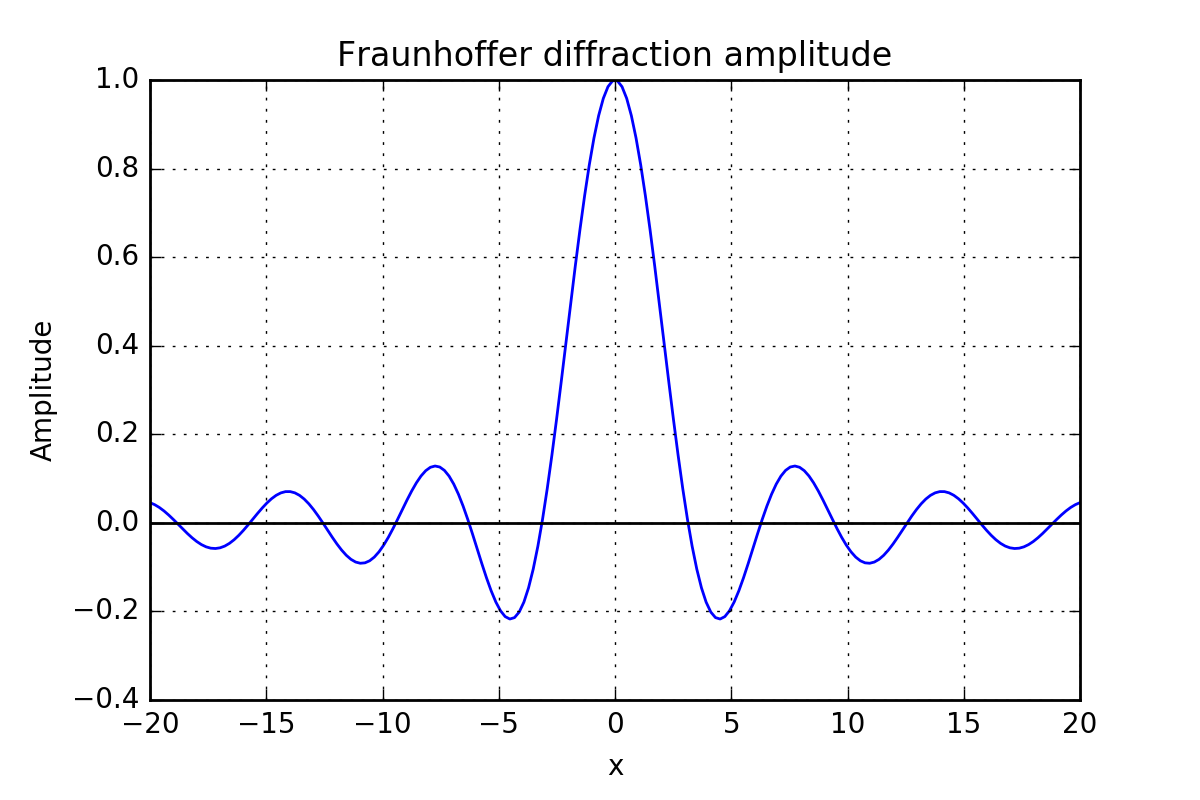
\includegraphics{fraun_amplitude}}
  \end{center}
  \caption{Fraunhoffer amplitude}
  \label{fig:fraun_amp}
\end{figure}

In order to find the diffraction angles of the maxima we solve for $\theta$ in Equation \ref{eq:fraun_x} such that,

\begin{equation}
\label{eq:diff_angle}
  \theta = \sin^{-1}\big(\frac{2x}{ka}}\big)
\end{equation}

The function $sin^{-1}{x}$ is defined for the interval, $-1 < x < 1$, which implies that the diffraction angles of the Fraunhoffer diffraction pattern are bounded by
such an interval. For Equation \ref{eq:diff_angle} we find the defining boundry by equating the function argument to 1 and solving for $x$. Hence,
the Fraunhoffer diffraction angles are defined for,

\begin{equation}
\label{eq:diff_anggle_interval}
  -\frac{ka}{2} < x < \frac{ka}{2}
\end{equation}

Thus we stop our root finding algorithm when the above condition is finally violated. In Figure \ref{fig:fraun_roots} we plot the Fraunhoffer Amplitude, its derivative
with respect to $x$ and the found roots to the right of the origin. Table \ref{tab:fraun_roots} summarizes the found roots and corresponding angles.


\begin{figure}[H]
  \begin{center}
    \scalebox{.8}{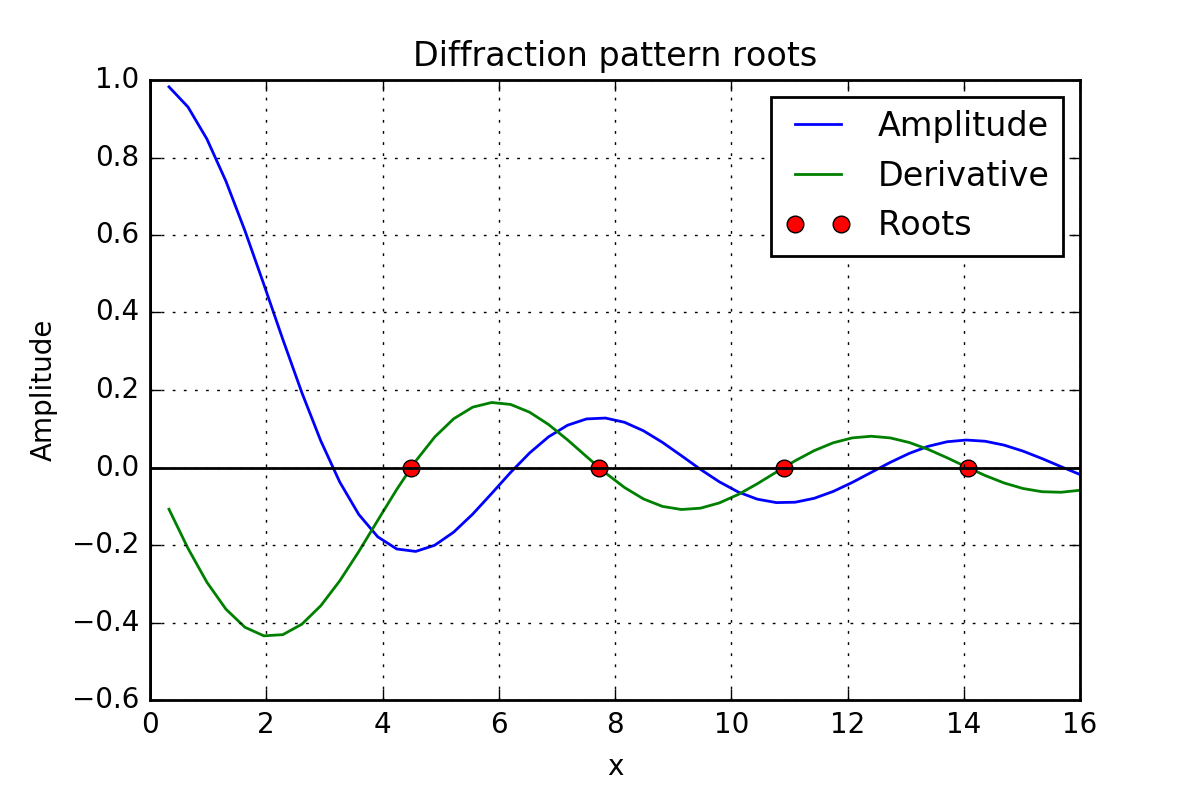
\includegraphics{fraun_root}}
  \end{center}
  \caption{Fraunhoffer diffraction pattern roots}
  \label{fig:fraun_roots}
\end{figure}

\begin{table}[H]
  \begin{center}
    \begin{tabular}{|c|c|c|c|}
      \hline
      Root & Angle(Radians) & Angle(Degrees) \\
      \hline
      4.493030 & 0.305737 & 17.52 \\
      \hline
      7.728195 & 0.544190 & 31.18 \\
      \hline
      10.906603 & 0.819277 & 46.94 \\
      \hline
      14.069672 & 1.230188 & 70.48 \\
      \hline
    \end{tabular}
  \end{center}
  \caption {Fraunhoffer roots and corresponding angles}
  \label{tab:fraun_roots}
\end{table}

Figure \ref{fig:fraun_int} shows the intensity of the Fraunhoffer diffraction with the locations of the ocurring maxima. Also, the given wavelength $\lambda = 589.29\;nm$
lies in the yellowish regime of the visible light spectrum. Thus, we also show the approximate expected diffraction pattern in a real life experiment.

\begin{figure}[H]
  \begin{center}
    \scalebox{.8}{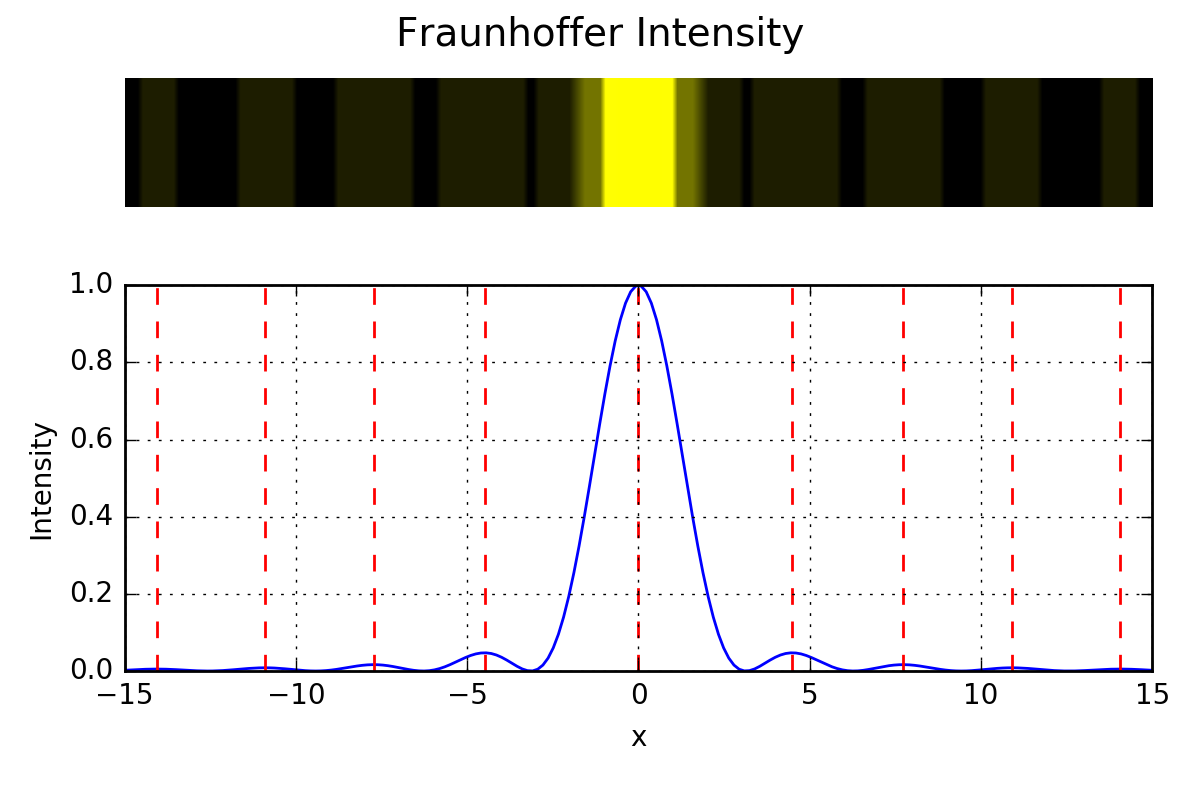
\includegraphics{fraun_int}}
  \end{center}
  \caption{Fraunhoffer intensity and diffraction pattern}
  \label{fig:fraun_int}
\end{figure}


\section{Matrix Computations}

Matrix computations are prevalent in many physical computations and numerical problems. In this exercise we explore
the GSL library subroutines for matrix computations and property extraction.

For these exercises, the following $3 \times 3$ matrix is used,

\begin{equation}
 \label{eq:mat}
 M = \begin{bmatrix}
       1 & 2 & 3 \\[0.3em]
       2 & 2 & 3 \\[0.3em]
       3 & 3 & 3 \\[0.3em]
      \end{bmatrix}
\end{equation}

In order to compute the inverse of the matrix, the LU Decomposition of matrix $M$ is found using the GSL subroutine \textit{gsl\textunderscore linalg\textunderscore LU\textunderscore decomp()}. Then,
we directly find the inverse using the subroutine \textit{gsl\textunderscore linalg\textunderscore LU\textunderscore invert()}. Below the result of such computations.

$$
 M^{-1} = \begin{bmatrix}
       -1 & 1 & 0 \\[0.3em]
       1 & -2 & 1 \\[0.3em]
       0 & 1 &  -\frac{2}{3}\\[0.3em]
      \end{bmatrix}
$$

Afterwards, we find the determinant of matrix $M$. From the previous computation we already have the LU decomposition, which is required for finding the determinant. Thus, to find the determinant,
we use \textit{gsl\textunderscore linalg\textunderscore LU\textunderscore det()}.

$$
 \label{eq:mat}
 \text{det(}M\text{)} = 3.0
$$

Finally, we find the eigenvalues and eigenvectors of matrix $M$. To carry out this computation the necessary GSL subroutine is \textit{gsl\textunderscore eigen\textunderscore symmv()}. Below are the
computed eigenvalues, followed by their corresponding eigenvectors.

$$
\lambda_{1} = -0.338922 \text{,}\quad
\lambda_{2} = -1.17762 \text{,}\quad
\lambda_{3} = 7.51654
$$

$$
e_{1} = \begin{bmatrix}
     0.42509 \\[0.3em]
     -0.829153 \\[0.3em]
     0.363048 \\[0.3em]
       \end{bmatrix}\text{,}\quad
e_{2} = \begin{bmatrix}
     0.765677 \\[0.3em]
     0.115485 \\[0.3em]
     -0.632774 \\[0.3em]
       \end{bmatrix}\text{,}\quad
e_{3} = \begin{bmatrix}
     0.482739 \\[0.3em]
     0.546963 \\[0.3em]
     0.683955 \\[0.3em]
       \end{bmatrix}
$$

We further investigate the computation time required to find the determinant of a matrix as the size of matrix increases. In Figure \ref{fig:det_plot}
the results of the experiment.

\begin{figure}[H]
  \begin{center}
    \scalebox{.8}{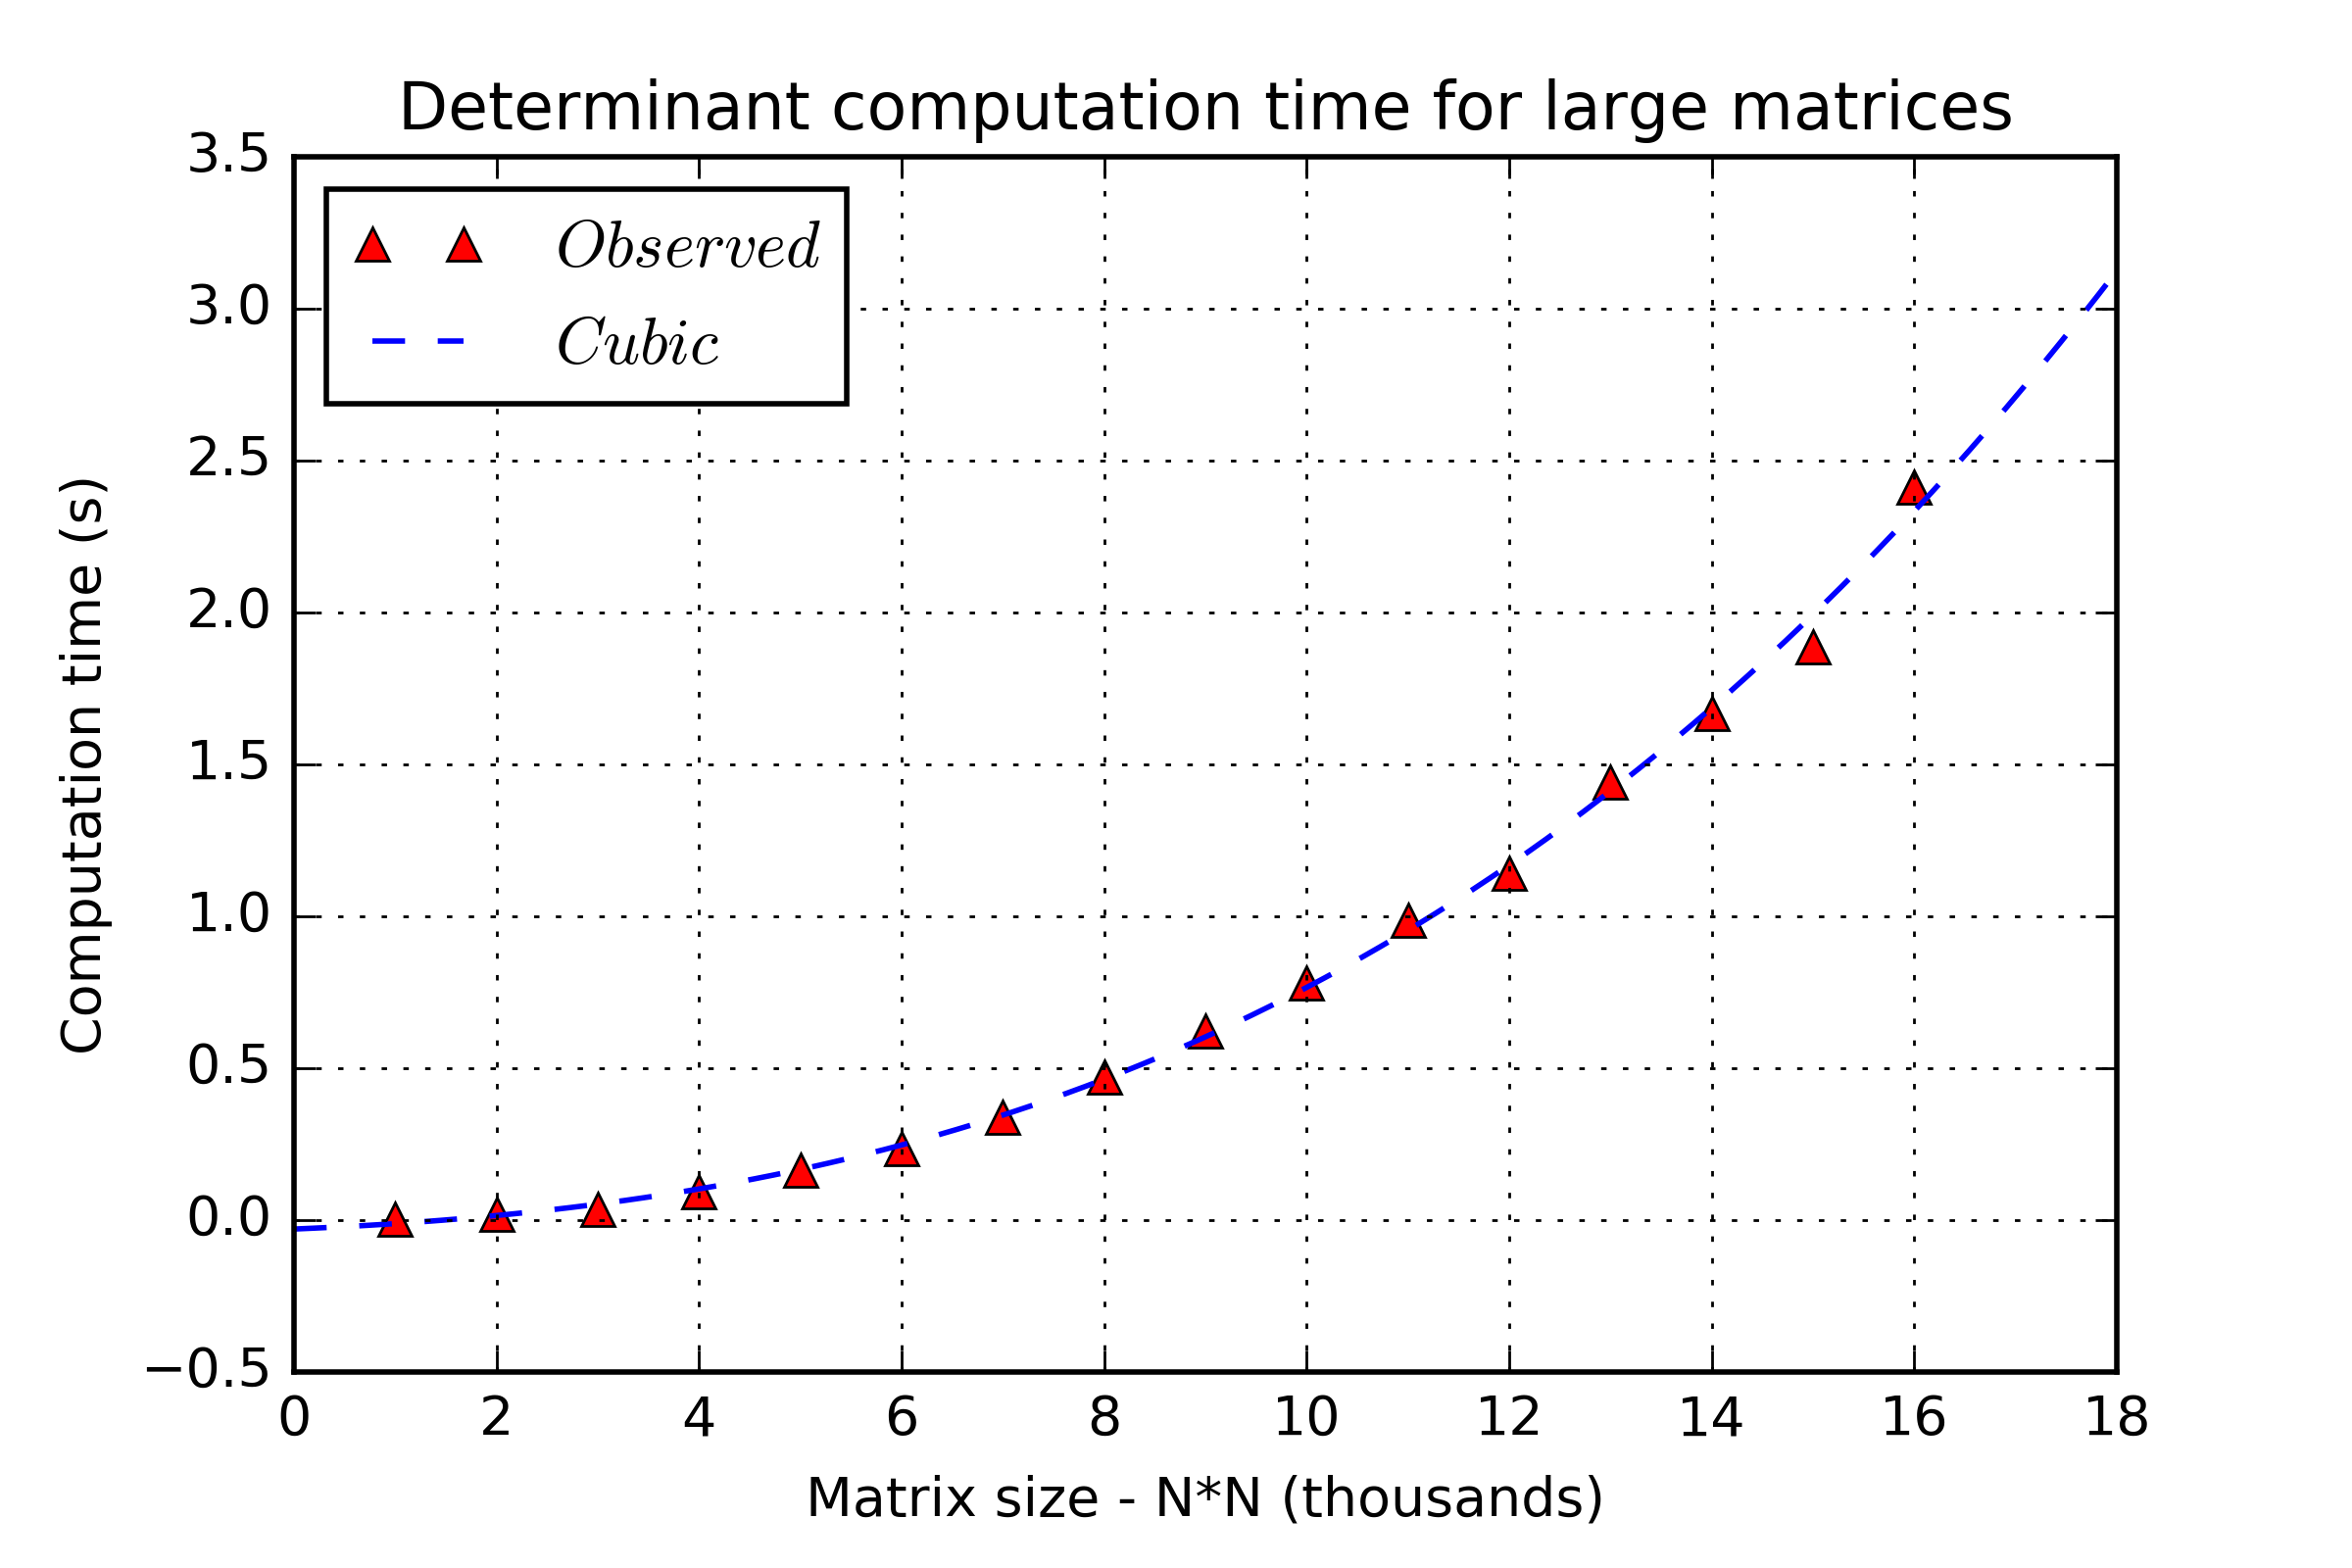
\includegraphics{det_plot}}
  \end{center}
  \caption{Determinant computation time for different matrix sizes}
  \label{fig:det_plot}
\end{figure}

As seen from the plot, the computation time closely scales as the cube of the matrix size.


\section{Method of over-relaxation}

For this section the code is implemented from scratch. We seek to numerically solve the Laplace equation for two dimensions. Laplace's
equation in two dimension is given by,


\begin{equation}
\label{eq:laplace_eq}
  \nabla^{2}u = 0
\end{equation}

where the Laplace operator $\nabla^{2} = \frac{\partial^2}{\partial x^2} + \frac{\partial^2}{\partial y^2}$. We consider a square $L \times L$ region with
temperature 100 at the top of the square and 0 everywhere else. The surrounding temperatures for a given site are represented as,

$$
u_{n} = u\big(x, y + h\big)
$$
$$
u_{w} = u\big(x - h, y\big)\text{,}\quad u_{c} = u\big(x, y\big)\text{,}\quad u_{e} = u\big(x + h, y\big) \\
$$
$$
u_{s} = u\big(x, y - h\big)
$$

By letting $h \rightarrow 0$, the surrounding temperatures can be approximated with a Taylor expansion such that the east and west neighbors are given by,

\begin{equation}
\label{eq:u_e}
  u_{e} \approx u_{c} + h\frac{\partial u}{\partial x} + \frac{1}{2}h^{2}\frac{\partial^2 u}{\partial x^2}
\end{equation}

\begin{equation}
\label{eq:u_w}
  u_{w} \approx u_{c} - h\frac{\partial u}{\partial x} + \frac{1}{2}h^{2}\frac{\partial^2 u}{\partial x^2}
\end{equation}

Combining Equations \ref{eq:u_e} and \ref{eq:u_w},

\begin{equation}
\label{eq:u_ew}
  u_{e} + u_{w} \approx 2u_{c} + h^{2}\frac{\partial^2 u}{\partial x^2}
\end{equation}

By similar treatment in the north and south directions we obtain,

\begin{equation}
\label{eq:u_ns}
  u_{n} + u_{s} \approx 2u_{c} + h^{2}\frac{\partial^2 u}{\partial y^2}
\end{equation}

Now we add Equations \ref{eq:u_ew} and \ref{eq:u_ns} such that,

$$
  u_{e} + u_{w} + u_{n} + u_{s} = 4u_{c} + h^{2}\bigg(\frac{\partial^2 u}{\partial x^2} + \frac{\partial^2 u}{\partial y^2}\bigg)
$$
$\Rightarrow$
$$
  \bigg(\frac{\partial^2 u}{\partial x^2} + \frac{\partial^2 u}{\partial y^2}\bigg) = \big(u_{e} + u_{w} + u_{n} + u_{s} - 4u_{c}\big)/h^{2}
$$

By Equation \ref{eq:laplace_eq},

$$
  \nabla^{2}u = \frac{\partial^2 u}{\partial x^2} + \frac{\partial^2 u}{\partial y^2} = 0
$$
$\Rightarrow$
$$
  \big(u_{e} + u_{w} + u_{n} + u_{s} - 4u_{c}\big)/h^{2} \approx 0
$$

Hence solving for $u_{c}$,

\begin{equation}
\label{eq:u_c_final}
 u_{c} \approx \big(u_{e} + u_{w} + u_{n} + u_{s}\big)/4
\end{equation}

The above equation suggests that in thermal equilibrium the temperature at a particular site is the average of its surrounding neighbors.


Now, to numerically solve the Laplace equation we make use of the Gauss-Seidel algorithm. Where, we construct an $L \times L$ lattice, set the corresponding
boundry conditions, and sweep through all sites in the lattice updating the temperatures as the average of its neighbors as suggested by Equation \ref{eq:update_uc}.
In this exercise the algorithm is ran continuosly until the average changes to the whole lattice is less than $1 \times 10^{-6}$. In other words, let $N = L \times L$ and
the change to a given site is given by $\Delta u_{i} = |u_{i, new} - u_{i, old}|$. Then the lattice is sweeped and updated until,

\begin{equation}
\label{eq:limit_uc}
  \Delta u_{avg} = \frac{\sum_{i=0}^{N} \Delta u_{i}}{N} < 1 \times 10^{-6}
\end{equation}


The theory of over-relaxation suggests that by introducing a relxation factor $f$ we can considerably speedup the convergence of the solution. Thus, by introducing the
relaxation factor we update a temperature as,

\begin{equation}
\label{eq:update_uc}
  u_{c, next} = \big(1 - f\big) \times u_{c} + f \times \big(u_{n} + u_{s} + u_{e} + u_{w}\big)/4
\end{equation}

We note that for $f = 1$ we end up with the Gauss-Seidel. Over-relxation works for $f > 1$ and the algorithm only converges for $f < 2$. Thus, the relaxation factor in this
exercise is bounded by the interval $1 \leq f < 2$. According to the theory, the optimal relxation factor for a lattice of size $L$ is given by,

\begin{equation}
\label{eq:f_opt}
  f_{opt} = 2 - 2\pi/L
\end{equation}

This optimal relxation factor guarantees the quickest convergence to the solution. The analytical solution for a $10\text{ cm}^2$ metal plate with the same
boundry conditions mentioned before is given by,

\begin{equation}
\label{eq:actual_t}
  T = \sum_{odd n} \frac{400}{n\pi \sinh{n\pi}}\sinh{\frac{n\pi}{10}\big(10 - y\big)}\sin{\frac{n\pi x}{10}}
\end{equation}

Thus we compare the eventual convergence of our simulated lattice to the analytical solution described above.

Below are the results of a simulated $ 500 \times 500$ lattice against the analytical solution. Both lattices and indifferentiable and assures we have
obtained adequete convergence.

\begin{figure}[H]
  \begin{center}
    \scalebox{.8}{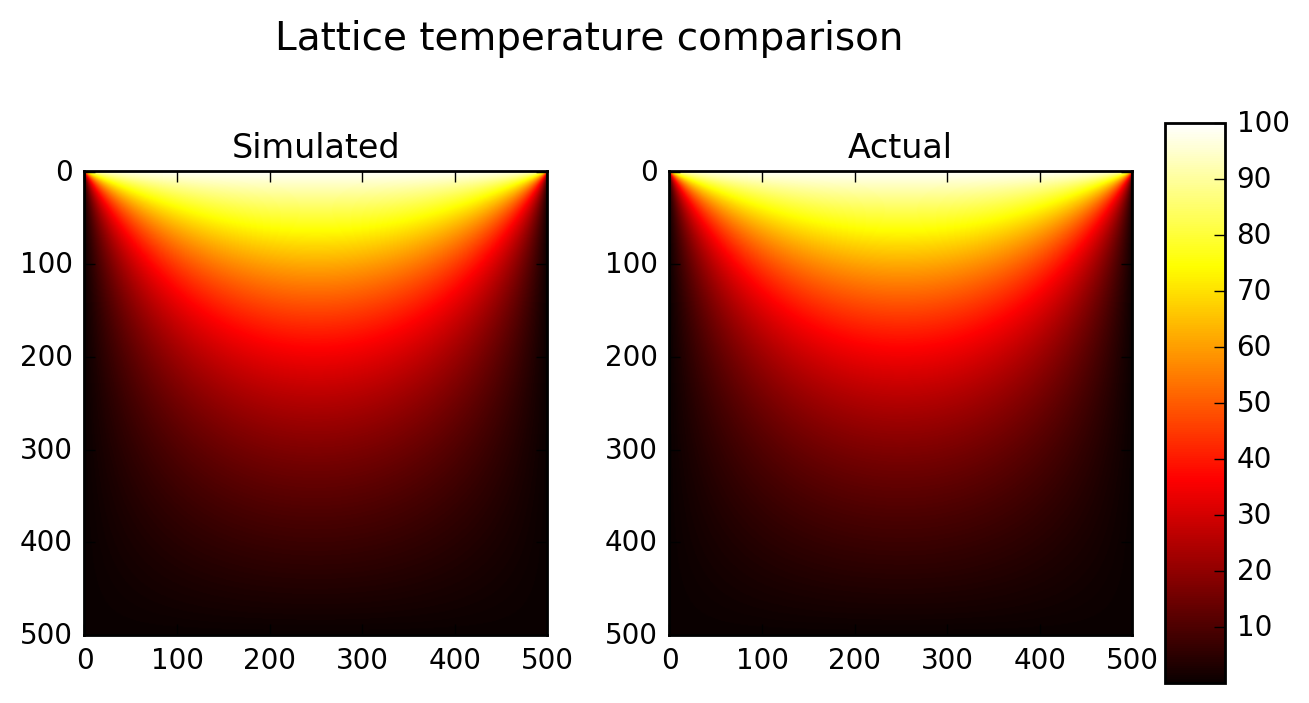
\includegraphics{temp_comp}}
  \end{center}
  \caption{Lattice temperature comparison for $500 \times 500$ lattice}
  \label{fig:lattice_comp}
\end{figure}

In order to test the theory of overrelaxation we count the number of iterations to converge to the desired accuracy for
a particular relaxation factor $f$. As seen in Figure \ref{fig:iter_plot}, as the relaxation factor increases, the number
of iterations drops considerably for lattices of size $L$. In order to test the theory for the optimal relaxation factor we
must zoom in to the region between 1.9 and 2.0 in Figure \ref{fig:iter_plot}.

\begin{figure}[H]
  \begin{center}
    \scalebox{.7}{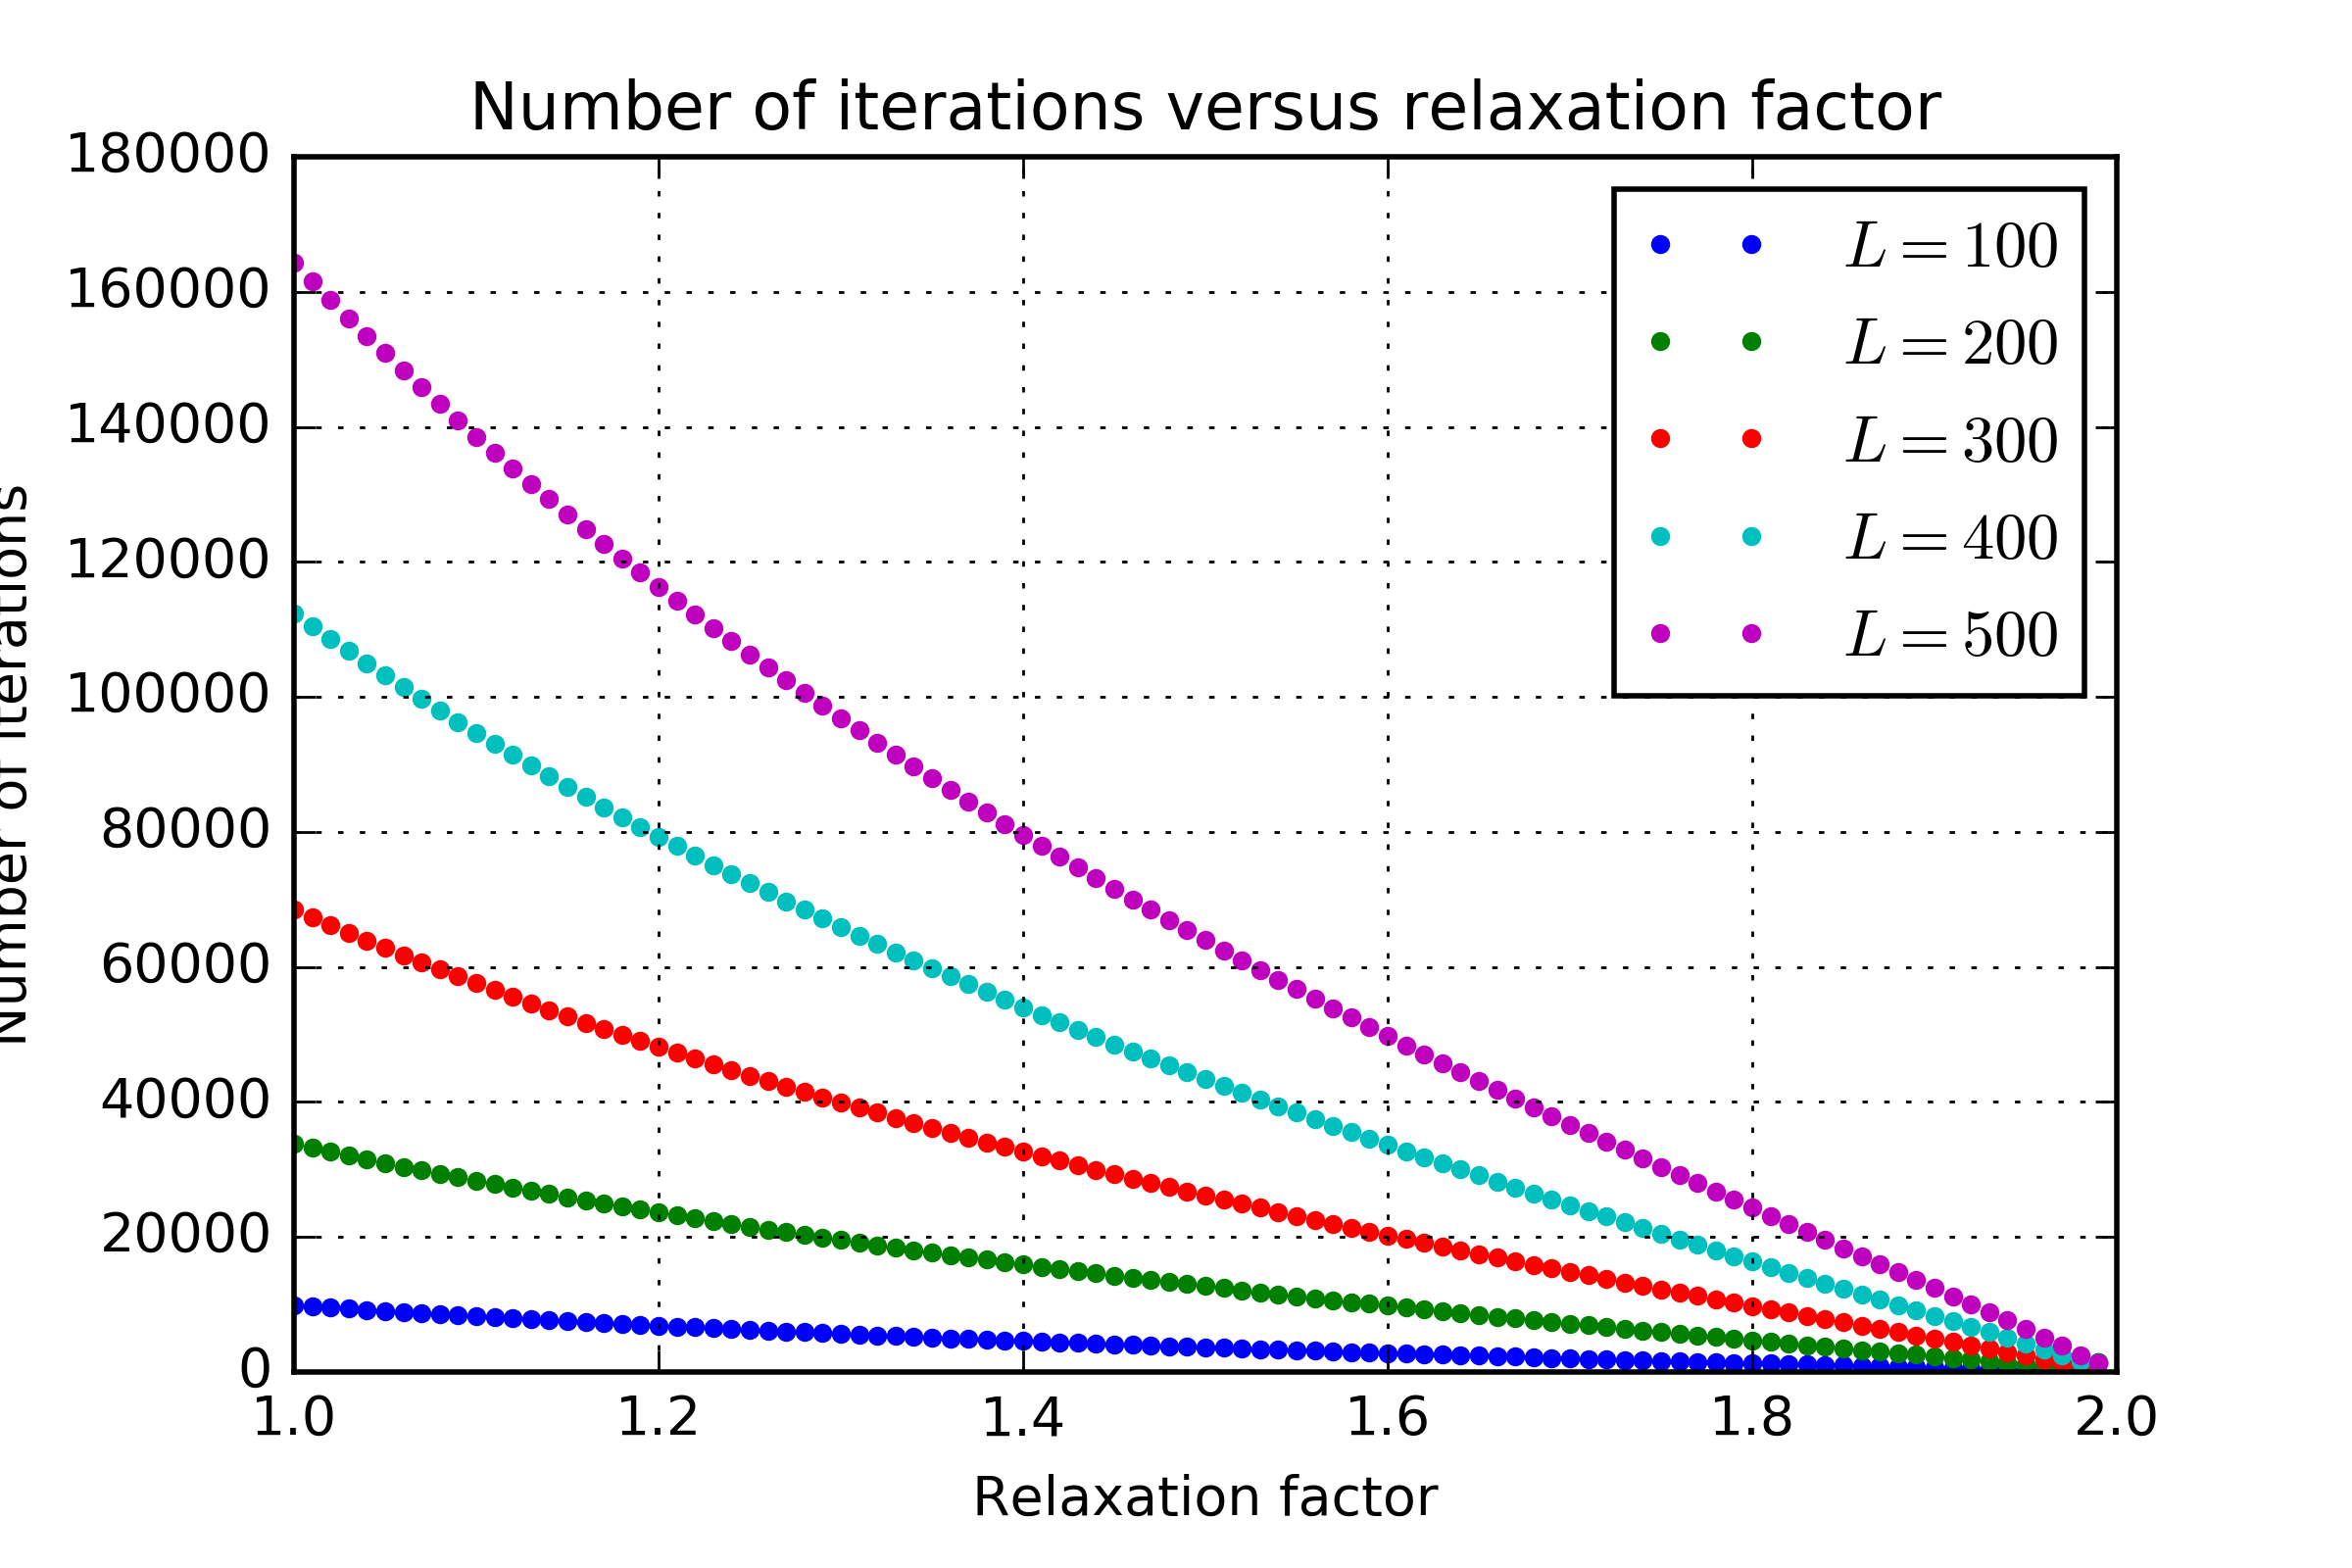
\includegraphics{iter_plot}}
  \end{center}
  \caption{Number of iterations to achieve desired accuracy as a function of the relaxation factor}
  \label{fig:iter_plot}
\end{figure}


\begin{figure}[H]
  \begin{center}
    \scalebox{.8}{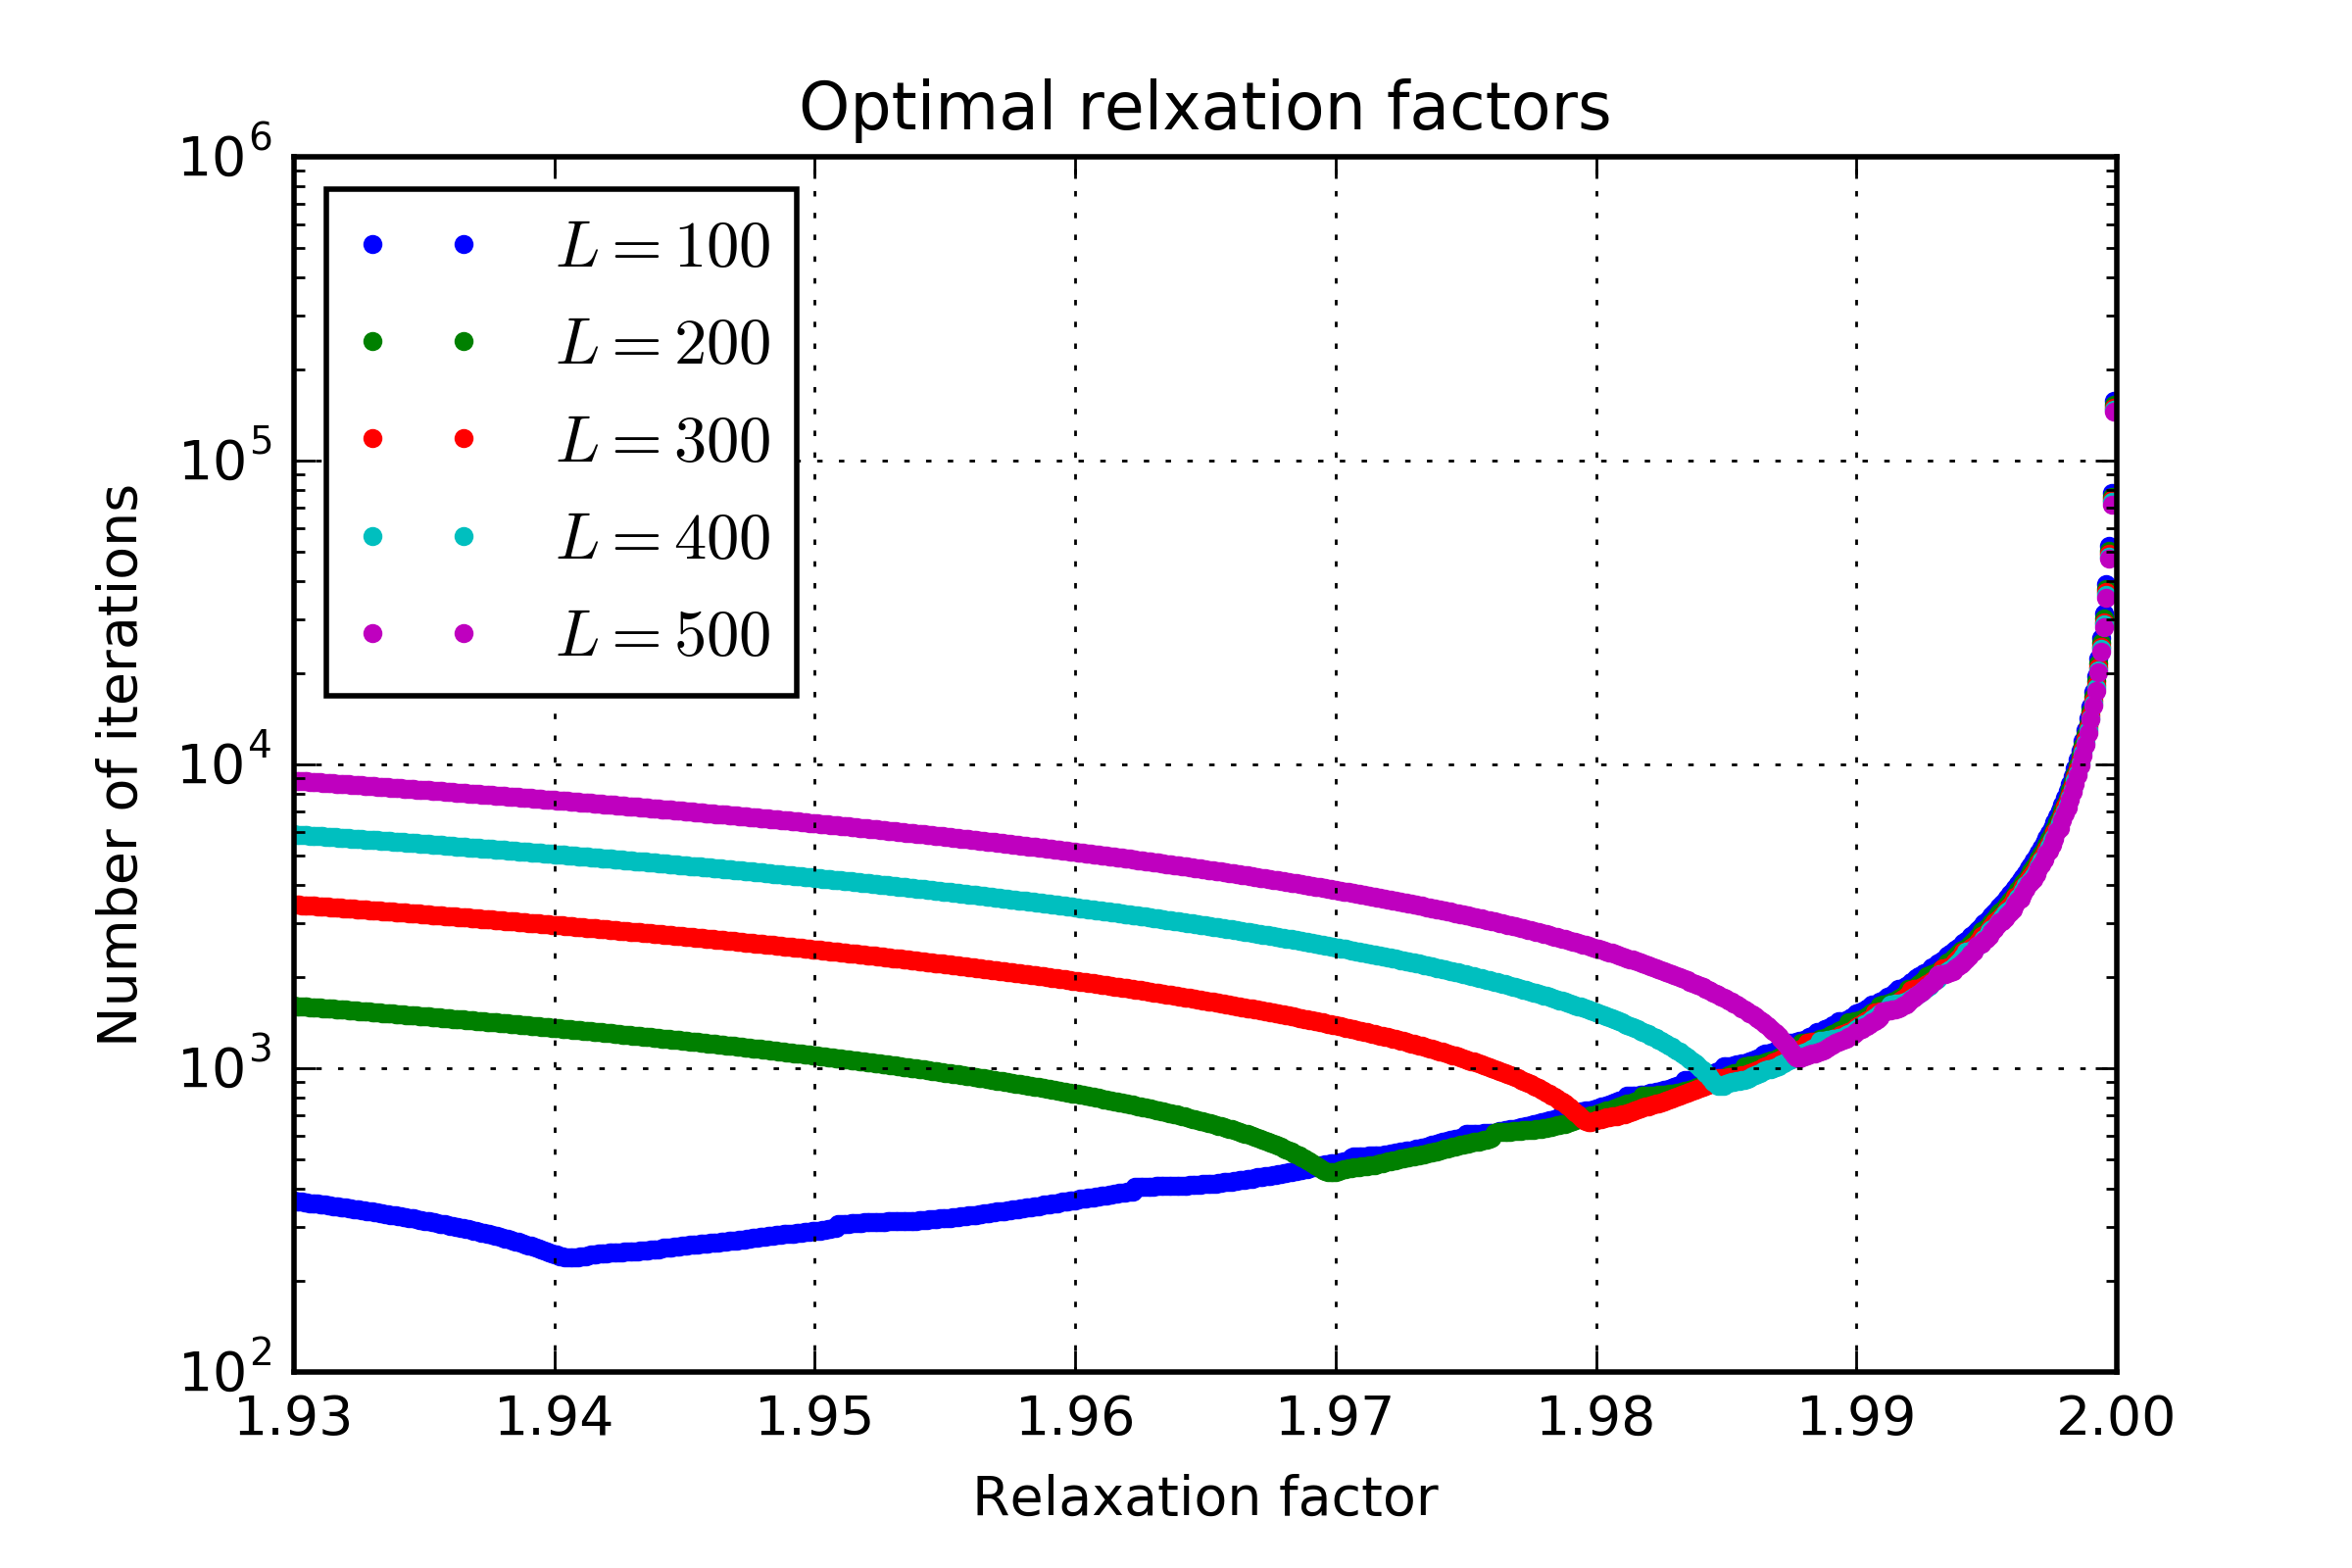
\includegraphics{iter_op_plot}}
  \end{center}
  \caption{Visualization of the optimal relxation factor for different lattice sizes}
  \label{fig:optimal_plot}
\end{figure}

As seen in Figure \ref{fig:optimal_plot} particular drops in the number of iterations seems to suggest there is some optimal relaxation factor as prescribed in
Equation \ref{eq:f_opt}. Also, as the theory suggests over-relaxation works for the interval $1 \leq f < 2$ and inspecting Figure \ref{fig:optimal_plot} around 2
we see how the number of iterations start to diverge. We find the relaxation factors that lead to the lowest number of iterations per lattice size and summarize
the data in Table \ref{tab:op_relax_factor}.

\begin{table}[H]
  \begin{center}
    \begin{tabular}{|c|c|c|c|}
      \hline
      Lattice size & Simulated & Predicted & $\%$ Error \\
      \hline
      100 &  1.941 & 1.937 & 0.2\%\\
      \hline
      200 & 1.9699 & 1.9686 & 0.07\% \\
      \hline
      300 &  1.9798 & 1.9791 &  0.04\% \\
      \hline
      400 & 1.9848 & 1.9843 &  0.03\% \\
      \hline
      500 & 1.9878 & 1.9874 &  0.02\% \\
      \hline
    \end{tabular}
  \end{center}
  \caption {Summary of found optimal relaxation factors $f_{opt}$}
  \label{tab:op_relax_factor}
\end{table}

The optimal relxation factor as suggested by the theory have been found to a satisfactory precision. In Table \ref{tab:relax_iter}
we summarize the performance obtained for each lattice size. The table shows the number of iterations for the Best, Average
and Worst case scenarios. As expected the best case always occurs exactly at the found relaxation factor. Whereas, the Worst case
occurs as $f$ gets closer to 2 where over-relaxation starts to diverge.

\begin{table}[H]
  \begin{center}
    \begin{tabular}{|c|c|c|c|}
      \hline
      Lattice size & Best Case & Avg. Case & Worst Case \\
      \hline
      100 & 240 & 1573 & 156548 \\
      \hline
      200 & 455 & 1952 & 152462 \\
      \hline
      300 & 665 & 2769 & 149434 \\
      \hline
      400 & 874 & 3931 & 146947 \\
      \hline
      500 & 1082 & 5397 & 144988 \\
      \hline
    \end{tabular}
  \end{center}
  \caption {Summary of solution performance for different Lattice sizes}
  \label{tab:relax_iter}
\end{table}


\section{Conclusion}

The GSL software library has been effectively used to solve some numerical problems such as the Fraunhoffer diffraction and matrix computations. Implementing the algorithms
provided by the library could have achieved the same results but would have consumed more time and could lead to unknown errors. The convinience that GSL provides to solve numerical
problems is unquestionable given its robustness and quantity of algorithms available.

We have also seen and verified the theory of over-relaxation for solving Laplace's equation. Not only is the theory correct but provides a useful optimization for speeding up the convergence
of a solution.

\begin{thebibliography}{9}

  \bibitem{gsl}
   GSL contributors. \emph{GNU Scientific Library} GNU, 9 Dec. 2016.

   \bibitem{hunter}
     Hunter, J. D.,
     \emph{Matplotlib: A 2D graphics environment}. Computing In Science \& Engineering, IEEE COMPUTER SOC

   \bibitem{fraun}
     Wikipedia contributors. \emph{Fraunhofer diffraction}. Wikipedia, The Free Encyclopedia. Wikipedia, The Free Encyclopedia, 24 Mar. 2017.

  \bibitem{latex}
	  Wikibooks contibutors,
	  \emph{Latex}. Wikibooks, The Free Textbook Project, 26 Dec. 2016



\end{thebibliography}
\end{document}
